%%%%%%%%%%%%%%%%%%%%%%%%%%%%%%%%%%%%%%%%%%%%%%%%%%%%%%%%%%%%%%%%%%
%        Contents: Bachelorarbeit, HS Fulda        %
%                          06.09.2022                        %
%---------------------------------------------------------%
%                     Implementierung.tex               %
%                        by Carina Möller                   %
%                    cary_moeller@gmx.de              %
%%%%%%%%%%%%%%%%%%%%%%%%%%%%%%%%%%%%%%%%%%%%%%%%%%%%%%%%%%%%%%%%%%

\chapter{Implementierung} \label{IM}
Im Folgenden werden zunächst ganz allgemein die bei der Implementierung verwendeten Sprachen und Bibliotheken vorgestellt und der In"~ und Output der Engine näher beleuchtet, bevor auf die konkrete Umsetzung der beiden generischen Ansätze aus Kapitel\nbs\ref{ED} und\nbs\ref{MD} eingegangen wird.

\section{Sprachen und Bibliotheken} \label{IA}

Bei \xblackout{p36} wird im Backend weitestgehend mit Java gearbeitet, während im Frontend TypeScript zum Einsatz kommt. Auch wenn langfristig immer mehr auf TypeScript umgestellt werden soll, fiel daher die Wahl der Programmiersprache auf Java. Dadurch kann die Transformationsengine nahtlos in die bestehende Struktur eingebunden werden und die Anzahl neuer Abhängigkeiten von externen Bibliotheken wird niedrig gehalten. Die Transformationsengine wurde als Maven"=Projekt aufgesetzt und verwendet Java\nbs8 als Version\nbs\cite[S.\;1--16]{java:lifesci}.

\subsection{JSON} \label{BibJSON}
Die Produktdaten liegen im JSON"=Format vor. JSON ist mittlerweile eines der weit verbreitetsten und gängigsten Datenaustauschformate. Da es jedoch keine native JSON"=Schnittstelle in Java gibt, wurden im Lauf der Zeit eine Vielzahl an open"=source Bibliotheken zur Verwendung von JSON entwickelt.  Sie dienen im Wesentlichen dazu, JSON zu verarbeiten, zu speichern oder auszutauschen. Ersteres wird durch das Parsen, Abfragen, Transformieren und Generieren von JSON"=Dokumenten ermöglicht, letzteres durch Serialisierung bzw. Deserialisierung, d.\,h. die Umwandlung eines Java"=Objekts in einen String im JSON"=Format bzw. die Rückrichtung. Jede API weist ihre Vor"~ und Nachteile auf und variiert in der Syntax sowie im Umfang. Durch die große Anzahl decken die Schnittstellen mit ihren individuellen Einsatzgebieten in Summe fast alle Anwendungsmöglichkeiten ab und bieten viel Flexibilität. Eine ausführliche Gegenüberstellung von vier exemplarischen Bibliotheken ist in\nbs\cite{json:libs1} zu finden, während\nbs\cite{json:libs2} 20 APIs bzgl. des Ein"~ und Ausgabeverhaltens vergleicht. In den Benchmarks\nbs\cite{json:bm1} und\nbs\cite{json:bm2} wird hingegen die Performanz gemessen. Eine Auswahl an Bibliotheken gestaffelt nach Popularität\footnote{gemessen an der Häufigkeit der Nutzung in anderen Artifakten aller verzeichneten Maven"=Repositories (auf \url{https://mvnrepository.com})} ist hier aufgelistet:
\begin{itemize}
\item \bib{Jackson} von Tatu Saloranta (2008)
\item \bib{Gson} von Google (2008)
\item \bib{org.json} von Douglas Crockford / Sean Leary (2010)
\item \bib{json-simple} von Fang Yidong / Davin Loegering (2008)
\item \bib{JSON-P} und \bib{JSON-B} aus der Jakarta EE\footnote{Jakarta EE, ehemals Java Platform, Enterprise Edition: Spezifikationen für Unternehmens"= und Webanwendungen, die auf der Java Standard Edition aufsetzen} (2019)
\end{itemize}
\bib{Jackson}\nbs\cite[S.\,323--403]{java:json} schneidet in den oben genannten Benchmarks leistungstechnisch besonders gut ab, während \bib{Gson} \nbs\cite[S.\,243--298]{java:json} im fehlerfreien Parsen beeindruckt. Beide Bibliotheken werden mit Abstand am häufigsten verwendet und bestechen durch ihre vielseitigen Funktionalitäten, insbesondere im Bereich der Serialisierung. Im Gegensatz dazu sind \bib{org.json} und \bib{json-simple}, wie der Name schon andeutet, leichtgewichtig und unkompliziert in der Verwendung, beschränken sich allerdings nur auf das Lesen und Schreiben. \bib{JSON-P} (Processing) und \bib{JSON-B} (Binding) sind als Standard in Jakarta eingebunden und können u.\,a. mit \bib{JsonPointer} arbeiten, vgl.\nbs\cite[S.\,21--34]{java:cls}.\\
In diesem Projekt wird JSON mittels \bib{Jackson} eingebunden. Die Bibliothek ist wie bereits erwähnt besonders populär, schnell und umfangreich und sie zeichnet sich durch regelmäßige Veröffentlichung neuer Releases aus, siehe\nbs\cite{jackson}. Außerdem wird sie bereits innerhalb der \xblackout{UDI Platform} verwendet, wodurch Einheitlichkeit erhalten werden kann. Ein für die Transformationsengine relevanter Nachteil besteht darin, dass die Navigation entlang bestimmter Pfade nur umständlich umgesetzt werden kann. Dafür unterstützt \bib{Jackson} allerdings das Prinzip der Datenbindung, was in Abschnitt\nbs\ref{IMD} genutzt wird. 

Natürlich muss auch die Bibliothek für die gewählte JSON"=Abfragesprache eingebunden werden, also in diesem Fall \bib{JMESPath} bzw. \bib{JSONata4Java}. Beide Schnittstellen unterstützen die Verwendung unter \bib{Jackson} (als auch \bib{Gson}), sodass es zu keinen Kompatibilitätsproblemen kommt.\\
In Ansatz\nbs\ref{MD} wird zusätzlich noch ein JSON"=Schema"=Validator für die YAML"=Datei einbunden. Hier gibt es ebenfalls viele verschiedene Bibliotheken zur Auswahl, die sich alle nicht wesentlich unterscheiden, außer in den Randbedingungen, die für Transformationsengine vernachlässigbar sind.

\subsection{Excel} \label{BibExcel}
Für die Bearbeitung von Excel"=Dateien in Java ist in der Regel die Bibliothek \bib{Apache POI} die erste Wahl. Die wenigen Alternativen bieten zum Teil eine höhere Geschwindigkeit und geringeren Speicherverbrauch, dafür muss der Benutzer aber an anderen Stellen Einschränkungen hinnehmen vgl.\nbs\cite{poi:alt}. Um die nahtlose Eingliederung in das bestehende System zu gewährleisten, wurde sich direkt für \bib{Apache POI} entschieden. Hiermit können nicht nur Excel"=Dokumente, sondern allgemein Microsoft Office"=Dateien dynamisch gelesen und geschrieben werden. Die Abkürzung \bib{POI} stand anfangs ironischerweise für "`Poor Obfuscation Implementation"', wurde aber später aus Marketinggründen fallengelassen. Heute ist \bib{Apache POI} eine extrem mächtige Bibliothek, die allen Anforderungen zur Erstellung der Excel"=Dateien innerhalb dieses Projektes gerecht wird. Einziges Manko ist die Bearbeitung sehr großer Arbeitsmappen mit über 50.000 Zeilen, wobei vergleichbare Bibliotheken zwangsläufig auch ab einem gewissen Punkt an ihre Grenzen stoßen. Damit der Heap"=Speicherplatz nicht überläuft, gibt es eine Streaming"=Erweiterung, bei der immer nur auf einen gleitenden Bereich von Zeilen Zugriff besteht. Dies bringt natürlich Nachteile mit sich, insbesondere bei der Formelauswertung, außerdem sind einige Funktionalitäten noch nicht implementiert, siehe\nbs\cite{poi}. Für die Transformationengine ist das Schreiben der Excel"=Datei via Streaming noch nicht nötig, aber für die \xblackout{UDI Platform} allgemein arbeitet \xblackout{p36} gerade an einer Umstellung für den Massen"=Upload von bis zu 10.000 Produkten gleichzeitig.

\subsection{Testen} \label{Tests}
Gerade im medizinischen Bereich sind Tests zur Qualitätssicherung von besonderer Bedeutung. Unter dem Stichwort "`GxP"' müssen nicht nur die Medizinprodukte selbst Richtlinien zur Sicherheit, Wirksamkeit und ihrer Verwendung erfüllen, sondern indirekt auch die zugrundeliegende Lieferkette, vgl.\nbs\cite{gxp}. Darunter fällt insbesondere \xblackout{p36} als IT"=Zulieferer. Als anerkannter Standardleitfaden für computergestützte Systeme dient der GAMP\,5\,Guide\nbs\cite{gxp:gamp}.\\
Zur Validierung der Software kommen dabei verschiedene Testarten zum Einsatz: von Modultests über Integrationstests und Funktions"~/Systemtests bis hin zu Akzeptanztests. Auf unterster Ebene wurden auch für dieses Projekt Modultests geschrieben, um die einzelnen Bestandteile der Transformationsengine lokal zu testen. Umgesetzt wurde dies mit \bib{JUnit\nbs4}, siehe dazu\nbs\cite{test:junit} und\nbs\cite[S.\,47--79]{test:quali}. Neben verschiedenen Testfällen für die jeweiligen Klassen mit ihren Methoden, wurde auch getestet wie viele Produkte in einem Zug in eine Excel"=Vorlage geschrieben werden können, bevor es zum Heap"=Overflow kommt. Darauf wird in Abschnitt\nbs\ref{MUT} noch näher eingegangen.

Das Logging läuft über die Fassade \bib{SLF4J} (Simple Logging Facade for Java, vgl.\nbs\cite{slf4j}), in welcher wiederum das Framework \bib{Log4j\nbs2} angewendet wird.
Zur Vereinfachung wird dabei das \bib{Project Lombok}\nbs\cite{lombok} verwendet, welches mit einer Annotation automatisch das gewünschte Log"=Feld für eine Klasse erzeugt. Des weiteren kommen \bib{Lombok}"=Annotationen an verschiedenen Stellen als Shortcuts für Getter, Setter und Null"=Checks zum Einsatz.

Damit sind bereits alle Abhängigkeiten erwähnt und die Maven"=Konfigurationsdatei \texttt{pom.xml} bleibt relativ überschaubar. Insbesondere sind viele der Bibliotheken ohnehin schon anderweitig in der \xblackout{UDI Platform} in Verwendung\nbs --\nbs dabei wurde darauf geachtet, dass die Versionen möglichst übereinstimmen. Die Bibliotheken sind in Tabelle\nbs\ref{tab:bib} zur Übersicht aufgelistet.

\begin{table}[htbp]
\centering
\begin{tabular}[c]{|l|l|l|r|} 
\hhline{----}
Bibliothek & groupId & artifactId & version\TBstrut\\
\hhline{====}
Apache POI & org.apache.poi & poi \& poi-ooxml & 4.1.2\Tstrut\\
Jackson & com.fasterxml.jackson.core & jackson-databind & 2.13.0\\
JMESPath & io.burt & jmespath-jackson & 0.5.1\\
JSONata & com.ibm.jsonata4java & JSONata4Java & 1.7.8\\
\makecell[l]{JSON Schema\\[-0.15cm] Validator} & com.networknt & \makecell[l]{json-schema-\\[-0.15cm] validator} & 1.0.70\\
JUnit & junit & junit & 4.12\\
Logging & org.apache.logging.log4j & \makecell[l]{log4j-core\\[-0.15cm] log4j-slf4j-impl} & 2.7\\
Project Lombok & org.projectlombok & lombok & 1.18.24\Bstrut\\
\hhline{----}
\end{tabular}
\caption{Überblick über die verwendeten Bibliotheken}\label{tab:bib}
\end{table}

\section[Ein- und Ausgabeparameter]{Ein- und Ausgabe}
Man kann sich die Transformationsengine als in sich geschlossene Blackbox vorstellen, die in der \xblackout{UDI Platform} zum Einsatz kommt. \\
Die Eingabeparameter sind dabei die Produktdaten als String im JSON"=Format sowie die Excel"=Vorlage. Bei Ansatz\nbs\ref{MD} ist zusätzlich noch die bereits erwähnte YAML"=Datei nötig, welche das Mapping zwischen den Produktdaten und der Excel"=Datei definiert. Die beiden Dokumente werden als InputStream übergeben. Der Konstruktor mit den beschriebenen Eingabeparametern der Klasse \texttt{TransformationEngine} ist im folgenden Code ab Zeile\nbs\ref{line:con} abgebildet.\\
Als Ausgabe wird ein OutputStream erzeugt, der die mit den im Mapping spezifizierten Produktdaten ausgefüllte Excel"=Datei enthält. Auch diese Methode ist im folgenden Quelltext\nbs\ref{code:te} ab Zeile\nbs\ref{line:out} dargestellt. 

\begin{lstlisting}[emph={inTemplate, inMapping, deviceData, outExcel, template, mapping, devices, filledTemplate}]
/**(*\label{line:con}*)
 * constructor for the transformation engine
 * 
 * Reads the Excel template of a specific agency via InputStream.
 * Reads the YAML file via InputStream that contains the mapping between the Excel sheet and the device data given by JSONata expressions.
 * Reads the device data via String that shall be filled into the template. It needs to be in a JSON format of an array containing a JSON object for each device with all of its data.
 *
 * @param inTemplate InputStream of the Excel template given by agency
 * @param inMapping InputStream of the YAML file describing the mapping between Excel template and device data
 * @param deviceData String in JSON format of an array of all device objects with their data
 * @throws TransformationException custom exception for any errors that specifically occur during the transformation
 */
public TransformationEngine($$@NonNull$$ InputStream inTemplate, $$@NonNull$$ InputStream inMapping, $$@NonNull$$ String deviceData) throws TransformationException {
	setTemplate(inTemplate);
	setMapping(inMapping);
	setDevices(deviceData);
}
\end{lstlisting}
\begin{lstlisting}[emph={inTemplate, inMapping, deviceData, outExcel, template, mapping, devices, filledTemplate}, firstnumber=last,
caption=Auszüge aus der Klasse \texttt{TransformationEngine}, label=code:te]
/** (*\label{line:out}*)
 * Populates the Excel template with the given device data based on the mapping information in the YAML file.
 * Writes the Excel workbook to the OutputStream, for example a file.
 * 
 * @param outExcel the OutputStream for the filled Excel template
 * @return OutputStream with the filled Excel template
 * @throws TransformationException custom exception for any errors that specifically occur during the transformation
 */
public OutputStream fillTemplateWithDevices($$@NonNull$$ OutputStream outExcel) throws TransformationException {
	this.filledTemplate = fillTemplate(template, mapping, devices);
	return writeExcel(filledTemplate, outExcel);
}
\end{lstlisting}


\section{Ansatz mit Excel-Datei} \label{IED}

Die Implementierung von Ansatz\nbs\ref{ED} mit der bearbeiteten Excel"=Datei ist im Sequenzdiagramm in Abbildung\nbs\ref{fig:seq1} grob dargestellt.

\begin{figure}[h]
 \centering
 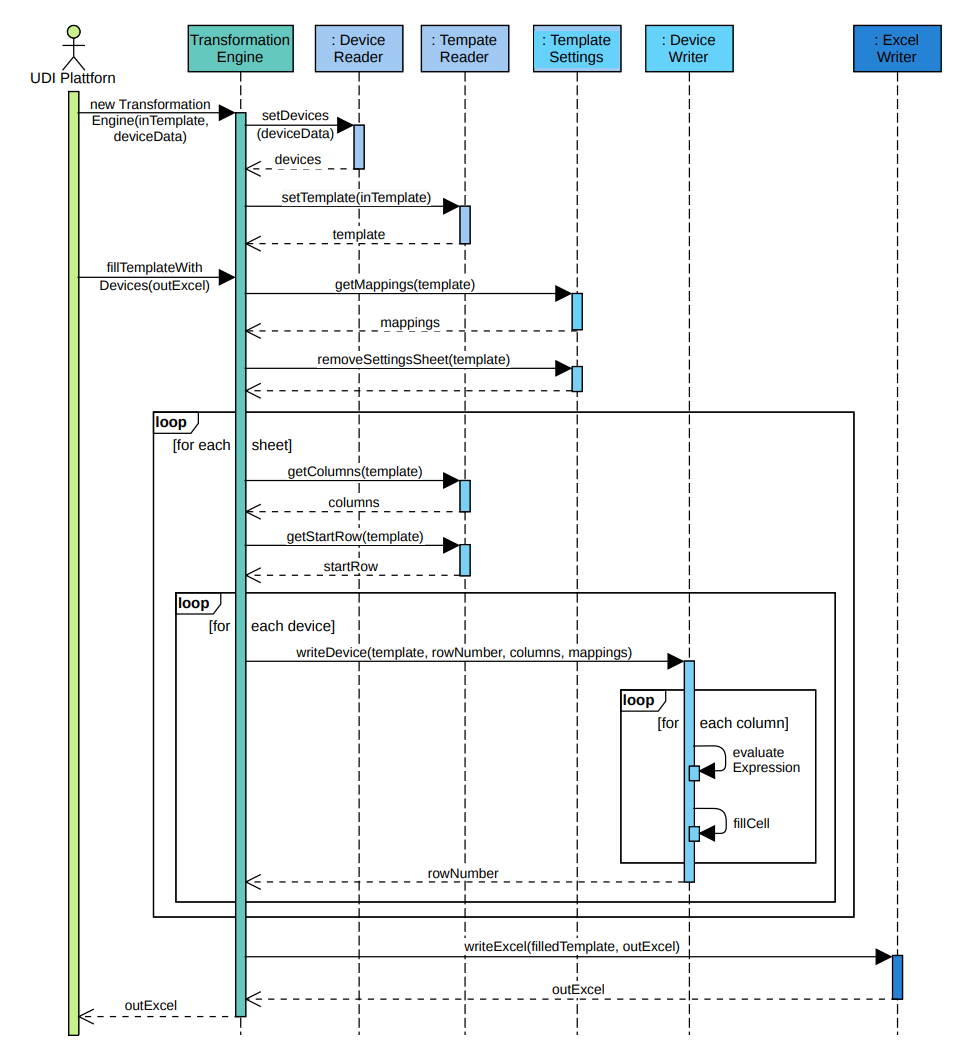
\includegraphics[width=0.95\textwidth]{Bilder/Sequenzdiagramm1}
 \caption[Sequenzdiagramm für Ansatz\nbs\ref{ED}]{Sequenzdiagramm}
 \label{fig:seq1}
\end{figure}

Im Konstruktor werden die Produktdaten \texttt{deviceData} eingelesen und als JsonNode abgespeichert. Außerdem wird die Excel"=Arbeitsmappe aus dem InputStream \texttt{inTemplate} mit der Bibliothek \bib{Apache POI} geladen. 

Bevor die Arbeitsblätter mit Daten gefüllt werden können, wird zunächst das Settings"=Arbeitsblatt ausgelesen und nach möglichen Mappings durchsucht. Diese werden in Hashtabellen gespeichert und im Anschluss kann das Settings"=Sheet gelöscht werden. Dies wurde bereits in Abschnitt\nbs\ref{zM} näher beschrieben und ist hier nur kurz skizziert.

Danach wird jedes Arbeitsblatt Zelle für Zelle nach Eingaben durchforstet, die mit \texttt{<} beginnen und \texttt{>} enden, um alle Spalten zu finden, welche mit Produktdaten gefüllt werden sollen. Der Code dafür ist im Quelltext\nbs\ref{code:col} abgebildet. 

\begin{lstlisting}[emph={columns, templateSheet, jmesPath, startRow, mandatory, row, cell, cellValue, message, e, column, colLetter, rowNumber, expression, log},
caption=Einlesen der Spalteninformationen in \texttt{TemplateReader}, label=code:col]
public HashMap<String, ColumnInfo> getColumns(Sheet templateSheet, JmesPath<JsonNode> jmesPath) throws TransformationException {
	HashMap<String, ColumnInfo> columns = new HashMap<String,ColumnInfo>();
	this.startRow = -1;

	for (Row row : templateSheet) {
		for (Cell cell : row) {
			if (cell.getCellType() == CellType.STRING) {
				String cellValue = cell.getRichStringCellValue().getString();
				if (cellValue.startsWith("<") && cellValue.endsWith(">")) { (*\label{line:found}*)
					//entry found
					cellValue = cellValue.substring(1, cellValue.length() - 1);
					
					//check if element is mandatory or cell can be left empty
					boolean mandatory = false;
					if (cellValue.statssWith("!")) {
						mandatory = true;
						cellValue = cellValue.substring(1, cellValue.length());
					}
					
					//parse JMESPath expression
					try {
						Expression<JsonNode> expression = jmesPath.compile(cellValue);
					} catch (ParseException e) {
						String colLetter = CellReference.convertNumToColString(cell.getColumnIndex());
						String message = String.format("JMESPath expression of sheet \"%s\", column %s cannot be parsed.\n%s",
									templateSheet.getSheetName(), colLetter, e.getMessage());
						log.error(message);
						throw new TransformationException(message, e);
					}

					//save all infos for this column
					ColumnInfo column = new ColumnInfo(cell.getColumnIndex(), mandatory, expression); (*\label{line:ci}*)
					columns.put(cellValue, column);

					checkIfRowsAlign(templateSheet, row.getRowNum());  (*\label{line:ra1}*)
				}
			}
		}
	}
	return columns;
}
\end{lstlisting}
Sobald eine Zelle gefunden wurde, die ein Spalteneintrag enthält (siehe Zeile\nbs\ref{line:found}), werden die entsprechenden Informationen verarbeitet und abgespeichert.
Wie man in Zeile\nbs\ref{line:ci} im folgenden Code sieht, wird nicht nur die Spaltennummer gespeichert, sondern auch die Angabe, ob die Spalte verpflichtend ist. Ebenso der kompilierte \bib{JMESPath}"=Ausdruck, mit dem später die geforderten Werte der einzelnen Produkte ermittelt werden können. Falls der Ausdruck fehlerhaft ist und nicht geparst werden kann, wird eine Exception ausgelöst, gefangen und in die eigens definierte \texttt{TransformationException} umgewandelt.\\
Zum Schluss in Zeile\nbs\ref{line:ra1} wird außerdem in der Methode \texttt{checkIfRowsAlign} die Excel"=Zeilennummer abgeglichen (siehe Quelltext\nbs\ref{code:col2}). Diese beschreibt die Start"=Zeile, in die der Inhalt des ersten Produkts eingetragen wird und womit die \bib{JMESPath}"=Ausdrücke aus der Vorlage überschrieben werden. Unterscheiden sich die Start"=Zeilen innerhalb eines Arbeitsblattes, wird ebenfalls eine \texttt{TransformationException} geworfen, weil die Einträge eines Datensatzes nicht alle in gerader Fluchtlinie (d.\,h. in einer Zeile) angeordnet sind.

\begin{lstlisting}[emph={columns, templateSheet, jmesPath, startRow, mandatory, row, cell, cellValue, message, e, column, colLetter, rowNumber, expression, log},
caption=Hilfsfunktion beim Einlesen der Spalteninformationen, label=code:col2]
private checkIfRowsAlign(Sheet templateSheet, int rowNumber) throws TransformationException; (*\label{line:ra2}*)
	switch (this.startRow) {
		case -1:				//first entry - initialize
			this.startRow = rowNumber;
			break;
		case rowNumber:	//all good
			break;
		default:				//no alignment - error
			String message = String.format("The starting rows for the different device data fields do not align in sheet \"%s\".",
						templateSheet.getSheetName());
			log.error(message);
			throw new TransformationException(message);
			break;
	}
} (*\label{line:ra3}*)
\end{lstlisting}

Obwohl über Blätter, Spalten und Zeilen iteriert wird, liegt der Aufwand im Bereich $\mathcal{O}(n)$, wobei $n$ die Anzahl der Spalten beschreibt bzw. umformuliert die Anzahl der von der Behörde geforderten Produktinformationen. Diese Anzahl wird nicht sonderlich groß, sondern bewegt sich im zwei"~ bis unteren dreistelligen Bereich\footnote{Datensatz von Behörden mit UDI"=System in \cite{udi:timelines}: näherungsweise Anzahl an geforderten Datenattributen -- Minimum: 13 (Singapur); Maximum: 130 (EU)}. Die Anzahl der Arbeitsblätter und nicht"=leeren Zeilen in einer unausgefüllten Vorlage ist daher vernachlässigbar klein und entsprechend verbraucht die Suche nach den Spalten, d.\,h. die Ausführung von \texttt{getColumns}, wenig Zeit. 

Nachdem alle Spalten"~ und Mapping"=Informationen vorliegen und ausgewertet sind, werden die einzelnen Produkte in die Vorlage geschrieben. Dies geschieht in der Klasse \texttt{DeviceWriter}. Hierbei wird nochmal über die Spalten iteriert. Die \bib{JMESPath}"=Ausdrücke werden auf das explizite Produkt angewendet und der so erhaltene Wert wird zunächst anhand der vorliegenden Mappings in die behördenspezifische Format"~ oder Formulierungsvorgabe umgewandelt. Der ggf. "`übersetzte"' Wert wird dann entsprechend seines Types in die Excel"=Zelle geschrieben. Dabei werden Wahrheitswerte, Zahlen und Text sowie Datumsangaben unterstützt. Für Letztere ist das Format allerdings aktuell fest vorgegeben\nbs --\nbs hier könnte man durch zusätzliche Angaben im Settings"=Arbeitsblatt behördenspezifische Wünsche inkludieren. 

Wie bereits erwähnt, ist in der Regel pro Spalte und Produkt nur genau ein Wert gefordert, aber es kann auch vorkommen, dass zu einem Produkt mehrere Informationen bzgl. einer Kategorie vorliegen, die in mehrere Excel"=Zeilen geschrieben werden müssen (siehe Abbildung\nbs\ref{fig:t3}). Der \bib{JMESPath}"=Ausdruck liefert in diesem Fall ein Array, deren einzelne Einträge jeweils eine eigene Excel"=Zeile erhalten. Hierbei ist wichtig, dass \texttt{null}"=Werte mitgegeben werden, falls ein Datenelement in einem Array nicht vorhanden sein sollte, sodass für ein Produkt die Länge des Arrays pro Kategorie in jeder Spalte gleich ist. Dadurch wird gewährleistet, dass jeweils alle Werte einer Zeile zueinander gehören. Standardmäßig werden Nullwerte bei einer \bib{JMESPath}"=Projektion allerdings herausgefiltert und nicht berücksichtigt. Um dies zu umgehen, kann man sich Multiselect"=Listen bedienen, die mit dem Pipe"=Operator dann im Nachgang wieder glättet werden. Als Beispiel kann man das komplexe Element \texttt{TradeNames} betrachten.
\begin{lstlisting}[language=json,caption={Beispiel eines komplexen Datenelements},label=code:comp]
{
    "TradeNames": [
        {
            "TradeName": "englishName",
            "TradeNameLanguage": "EN"
        },
        {
(*\label{line:nol}*)            "TradeName": "noLanguageGiven"
        },
        {
            "TradeName": "deutscherName",
            "TradeNameLanguage": "DE"
        }
    ],
    (*\color{black}$\ldots$*)
}
\end{lstlisting}
Um für jedes Objekt eine neue Zeile zu erzeugen, in der sowohl \texttt{TradeName} als auch \texttt{TradeNameLanguage} in einer eigenen Spalte angegeben werden, bieten sich die folgenden \bib{JMESPath}"=Ausdrücke an:
\begin{itemize}
\item{\texttt{<TradeNames[].[TradeName] | []>}}
\item{\texttt{<TradeNames[].[TradeNameLanguage] | []>}}
\end{itemize}
Durch die zusätzlichen eckigen Klammern um die Datenelemente \texttt{TradeName} und \texttt{TradeNameLanguage} wird anstatt einer normalen Projektion eine Multiselect"=Liste erzeugt, die in diesem Fall aus ein"=elementigen Arrays besteht, weil nur ein Datenelement gesucht ist. Jedes Auswertungsteilergebnis ist dabei enthalten, auch wenn es \texttt{null} beträgt\nbs --\nbs in diesem Beispiel die nicht vorhandene Angabe der Sprache im zweiten Objekt (Zeile\nbs\ref{line:nol}). Mit \texttt{|[]} wird das erzeugte Array von Arrays wieder geglättet. Alternativ kann mit der eingebauten Funktion \texttt{map} gearbeitet werden. Der Ausdruck \texttt{map(\&TradeNameLanguage, TradeNames[])} führt zu demselben Ergebnis, da auch hier eine neue Liste erzeugt wird, die die gleiche Länge wie die ursprüngliche Liste hat. Jedes Objekt in \texttt{TradeNames} wird auf die \texttt{TradeNameLanguage} abgebildet, falls vorhanden\nbs --\nbs ansonsten auf \texttt{null}. Im Excel"=Template wird der Nullwert dann als leere Zelle interpretiert. 

Liegen fehlerhafte Produktdaten vor oder können \bib{JMESPath}"=Ausdrücke nicht interpretiert werden, bricht das Programm mit einer Fehlermeldung ab und die Informationen zum Produkt bzw. zur Spalte im Arbeitsblatt werden geloggt. Ursprünglich war die Logik so, dass Produkte mit Datenfehlern (z.\,B. ein fehlender, verpflichtender Wert) aus der Excel"=Vorlage gelöscht und geloggt, alle restlichen Produkte aber eingetragen wurden. Dadurch konnte immer eine valide Excel"=Datei erzeugt werden, die möglicherweise aber nur zu einem Bruchteil ausgefüllt war. Die Rücksprache im Team ergab, dass das erfolgreiche Durchlaufen trotz einzelner Fehler dazu führt, dass diese übersehen werden. Anstatt lediglich Einträge im Log zu hinterlassen, wird nun eine Exception geworfen. 

Die Implementation des \texttt{DeviceWriters}, um die Daten eines Produktes in die Arbeitsmappe zu schreiben, folgt bei beiden Ansätzen identischen Prinzipien. Ansatz\nbs\ref{IMD} ist etwas umfangreicher und es wurden einige Details optimiert, daher wird zur Veranschaulichung an dieser Stelle auf das später folgende Aktivitätsdiagramm\nbs\ref{fig:akt1} verwiesen. 

Konnten alle Produktdaten erfolgreich in die Arbeitsmappe eingetragen werden, wird das ausgefüllte Excel"=Template in der Klasse \texttt{ExcelWriter} in einen OutputStream geschrieben. Dabei kann es sich beispielsweise um eine Datei handeln, die dann erzeugt wird. 




%\clearpage

\section{Ansatz mit Mapping-Datei} \label{IMD}

Die Implementierung für den Ansatz mit der extra YAML"=Datei für die Projektion von Produktdaten in die Excel"=Datei ist in Abbildung\nbs\ref{fig:seq2} in einem Sequenzdiagramm dargestellt. Er ist ähnlich aufgebaut wie Ansatz\nbs\ref{IED}. Im Konstruktor werden wie bisher die Excel"=Vorlage geladen und die Produktdaten deserialisiert. Zusätzlich wird nun die Mapping"=Datei eingelesen und direkt validiert (siehe Abschnitt\nbs\ref{JSch}). Um die Produktdaten in die Arbeitsmappe zu schreiben, wird ebenfalls wieder über die Arbeitsblätter, die Produkte und die einzelnen Spalten iteriert. Dies geschieht in der Klasse \texttt{DeviceWriter}. 

\begin{figure}[h]
 \centering
 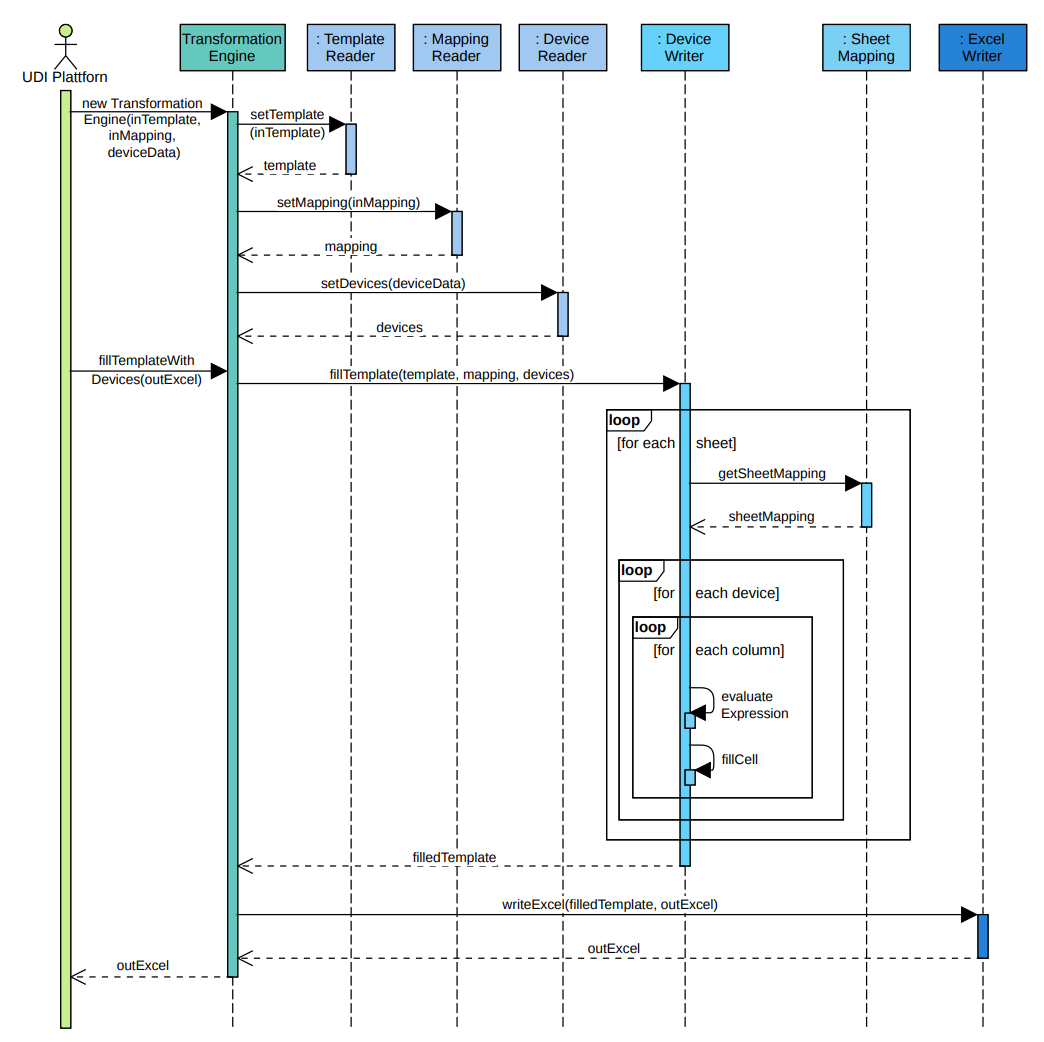
\includegraphics[width=0.95\textwidth]{Bilder/Sequenzdiagramm2}
 \caption[Sequenzdiagramm für Ansatz\nbs\ref{MD}]{Sequenzdiagramm}
 \label{fig:seq2}
\end{figure}

Eine interne Verbesserung zur Implementierung des vorherigen Ansatzes besteht darin, dass die Produktdaten, die auf behördenspezifische Werte abgebildet werden sollen, direkt als erstes vor den verschiedenen Schleifendurchläufen transformiert werden. Das gilt auch für die Datums"~ und Zeitformate. Dabei wird für jedes gewünschte Excel"=Format ein \texttt{CellStyle} angelegt, in einer Hashtabelle gespeichert und später auf diejenigen Zellen angewendet, die ein Datum im angegebenen Format enthalten (sollen). 
Für jeden in der Mapping"=Datei angegebenen Arbeitsblatt"=Titel werden die folgenden vier Schritte durchgeführt: 
\begin{enumerate}
\item Das zugehörige Arbeitsblatt in der Excel"=Vorlage suchen: Kann kein Arbeitsblatt mit dem angegebenen Namen gefunden werden, wird ein Fehler geworfen und die Transformationsengine bricht ab.
\item Die Angaben zum Arbeitsblatt aus der Mapping"=Datei per Datenbindung in ein Objekt der Klasse \texttt{SheetMapping} übertragen: Hierauf wird im folgenden Abschnitt\nbs\ref{DB} noch näher eingegangen. 
\item Die Variablen aus \texttt{SheetMapping} abrufen, unter anderem die Startzeile, die verschiedenen Spaltennamen mit deren \bib{JSONata}"=Ausdrücken sowie eine Liste aller verpflichtenden Spalten: Wurden dabei syntaktisch falsche Werte übergeben, wird ebenfalls ein Fehler geworden. 
\item Jedes Produkt in eine oder ggf. mehrere Zeilen des Excel"=Arbeitsblatts schreiben: Dabei wird wie in Kapitel\nbs\ref{ED} vorgegangen, indem spaltenweise der \bib{JSONata}"=Ausdruck ermittelt und dann im richtigen Format in die passende Zelle geschrieben wird. Dies wird in Abschnitt\nbs\ref{WOD} erläutert.
\end{enumerate}

\subsection[Datenbindung]{Datenbindung in SheetMapping}\label{DB}
Alle JSON"=Daten zu einem Arbeitsblatt werden dank der Bibliothek \bib{Jackson} an eine Instanz der Klasse \texttt{SheetMapping} gebunden, wie der Codeausschnitt\nbs\ref{code:db} zeigt. Man spricht hier von Daten"=Deserialisierung, da JSON"=Knoten in Java"=Objekte umgewandelt werden. 
Die Datenbindung an ein Objekt hat gegenüber der Speicherung im Baummodell den Vorteil, dass Abfragen deutlich bequemer durchführbar sind und einfacher mit den Daten gearbeitet werden kann. Anstatt wiederholt die Pfade des Baumes abzulaufen, können Parameter direkt referenziert werden.

\begin{lstlisting}[emph={jsonReader}]
ObjectMapper jsonReader = new ObjectMapper();
jsonReader
		.enable(DeserializationFeature.ACCEPT_EMPTY_STRING_AS_NULL_OBJECT);
\end{lstlisting}
\begin{lstlisting}[emph={jsonReader, sheetName, injextableValues, e, message, sheetMappings, log}, firstnumber=last, caption={Datenbindung für Arbeitsblätter der Mapping-Datei}, label=code:db]
private SheetMapping getSheetMapping(ObjectMapper jsonReader, String sheetName) throws TransformationException {
	InjectableValues injectableValues = (*\label{line:sn}*)
			new InjectableValues.Std().addValue(String.class, sheetName);
	try {
		return jsonReader
				.reader(injectableValues)
				.treeToValue(sheetMappings.get(sheetName), SheetMapping.class);
	} catch (JsonProcessingException | IllegalArgumentException e) {
		String message = String.format("Sheet called \"%s\" could not be filled, because the mapping cannot be parsed properly.", sheetName);
		log.error(message);
		throw new TransformationException(message, e);
	}
}
\end{lstlisting}
Umgesetzt wird die Anbindung durch Annotationen in der Klasse \texttt{SheetMapping}. Mit \texttt{@JacksonInject} wird der Name des Arbeitsblatts zur Klasse hinzugefügt, um diese Info den Fehlermeldungen mitgeben zu können. Dies wird in Zeile\nbs\ref{line:sn} im Code\nbs\ref{code:db} vorbereitet. Mit \texttt{@JsonProperty} werden alle weiteren Attribute gesetzt, die im Anschluss aufgelistet sind. 
\begin{itemize}
\item die Kategorie \texttt{category} als \texttt{String}:\\
Falls kein komplexes Datenelement angegeben wurde, auf welches sich das Arbeitsblatt bezieht, beträgt der Wert \texttt{null}. 
\item die Startzeile \texttt{row} als \texttt{Integer}:\\
Die Zeile muss größer als 0 sein, ansonsten bricht die Transformationsengine mit einer Fehlermeldung ab. Außerdem wird sie um eins reduziert, da die Bibliothek \bib{Apache POI} mit 0"=basierten Zeilennummern arbeitet, während die Zeilen in Excel bei 1 beginnen. 
\item die Spalten \texttt{columns} als \texttt{HashMap <String, String>} mit dem Spaltennamen als Schlüssel und dem \bib{JSONata}"=Ausdruck als Wert:\\
In der zugehörigen Getter"=Methode werden die Spaltennamen zunächst auf syntaktische Korrektheit überprüft (1-2 Buchstaben von A bis Z) und dann in die entsprechende 0"=basierte Spaltenzahl umgewandelt, mit welcher \bib{Apache POI} rechnet. Die Funktion ist im Code\nbs\ref{code:sgcol} in Zeile\nbs\ref{line:pc1}--\nbs\ref{line:pc2} dargestellt. Außerdem werden die \bib{JSONata}"=Ausdrücke mittels der Bibliothek \bib{JSONata4Java} geparsed und in \texttt{Expressions} umgewandelt. So wird also der Typ \texttt{Map <Integer, Expressions>} zurückgegeben. Tritt ein Fehler im Spaltennamen oder während des \bib{JSONata} Parsens auf, wird eine \texttt{TransformationException} geworfen.
\item die verpflichtenden Spalten \texttt{mandatoryColumns} als \texttt{HashSet <String>}:\\
Bevor die Menge der Spalten herausgegeben wird, werden auch hier die Spaltennamen in Zahlen, beginnend bei 0, umgerechnet und gegebenenfalls ein Fehler geworfen.   
\end{itemize}
Im folgenden Codeausschnitt\nbs\ref{code:sgcol} ist exemplarisch die Implementierung für die obligatorischen Spalten dargestellt. Alle gewöhnlichen Setter"~ und Getter"=Methoden ohne besondere Funktionalitäten werden einfachheitshalber mit Hilfe von \bib{Lombok}"=Annotationen deklariert, wie z.\,B. in Zeile\nbs\ref{line:setter}.
\begin{lstlisting}[emph={mandatoryColumns, columnLetter, mandatoryColumnsParsed, message, columnNumber, sheetName, log},
caption=Setter / Getter für verbindliche Spalten in \texttt{SheetMapping}, label=code:sgcol]
$$@JsonProperty$$("mandatoryColumns")
$$@Setter$$ (*\label{line:setter}*)
private Set<String> mandatoryColumns = new HashSet<String>();

//Getter
public Set<Integer> getParsedMandatoryColumns() throws TransformationException {
	Set<Integer> mandatoryColumnsParsed = new HashSet<Integer>();
	mandatoryColumns.forEach((columnLetter) -> {
		mandatoryColumnsParsed.add(parseCol(columnLetter));
	});
	return mandatoryColumnsParsed;
}

private Integer parseCol(String columnLetter) throws TransformationException { (*\label{line:pc1}*)
	columnLetter = columnLetter.toUpperCase();
	if (!columnLetter.matches("[A-Z]{1,2}")) {
		String message = String.format(
				"Yaml file describing agency template is not filled correctly: in sheet \"%s\", column %s is not a valid excel column name.",
				sheetName, columnLetter);
		log.error(message);
		throw new TransformationException(message);
	}
	int columnNumber = 0;
	for (int i = 0; i < columnLetter.length(); i++) {
		columnNumber = columnNumber * 26 + columnLetter.charAt(i) - 'A' + 1;
	}
	return columnNumber - 1;
} (*\label{line:pc2}*)
\end{lstlisting}
Die \texttt{TransformationException} ist eine benutzerdefinierte Ausnahme (siehe dazu\nbs\cite[S.\,32f]{java:lifesci} und\nbs\cite[S.\,309--338]{java:tut}), welche möglichst alle checked Exceptions zusammenfasst, die bei der Transformation entstehen können. Ausgenommen sind ungeprüfte Laufzeit"=Fehler. NullPointer"=Exceptions werden mittels \bib{Lombok} erzeugt, falls ein Eingabeparameter \texttt{null} ist. Betrachtet man die Transformationsengine im Zusammenspiel mit der restlichen Plattform, wird so direkt ersichtlich, dass ein Fehler innerhalb der Transformationsengine aufgetreten ist und im Log kann die genaue Ursache nachgelesen werden. 

\subsection{Produktdaten schreiben}\label{WOD}
Die spaltenweise Auswertung des \bib{JSONata}"=Ausdrucks und das Füllen der Zelle in der Excel"=Vorlage funktioniert ganz anlog zu Abschnitt\nbs\ref{IED}. Es ergibt sich das Aktivitätsdiagramm aus Abbildung\nbs\ref{fig:akt1} für die Methode \texttt{writeOneDevice} der Klasse \texttt{DeviceWriter}, um\nbs --\nbs wie der Name schon sagt\nbs --\nbs die Daten zu einem Produkt in ein Arbeitsblatt zu schreiben. 

\begin{figure}[!hbt]
 \centering
 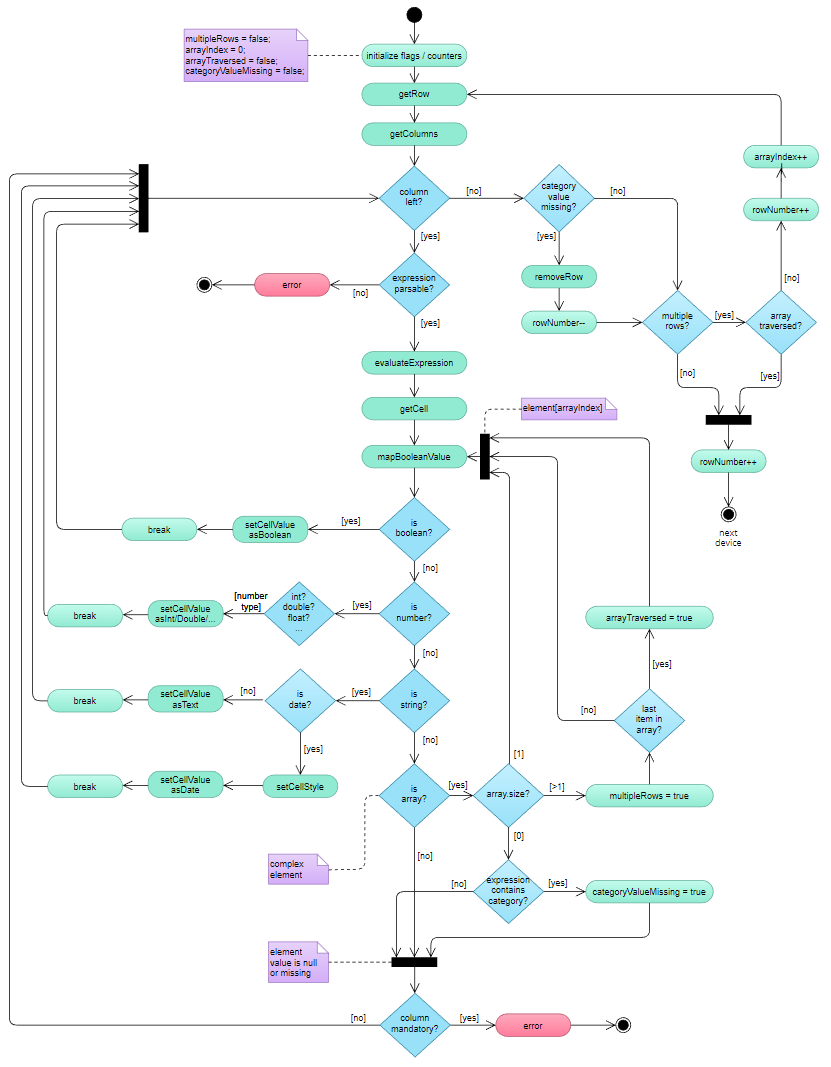
\includegraphics[width=\textwidth]{Bilder/Aktivitaetsdiagramm}
 \caption[Aktivitätsdiagramm für \texttt{writeOneDevice} aus Ansatz\nbs\ref{MD}]{Aktivitätsdiagramm für \texttt{writeOneDevice}}
 \label{fig:akt1}
\end{figure}

Um den Prozess im Aktivitätsdiagramm nachvollziehen zu können, wird zunächst der Unterschied zwischen einfachen und komplexen Datenelementen näher erläutert. 
Einfache Datenelemente stehen in einer 1\,:\,1"=Beziehung zum Produkt, das heißt es liegt nur eine einzige Ausprägung vor, die dem Datenelement zugeordnet ist. Dies kann als String, Zahl oder Wahrheitswert sein. Ein Spezialfall bildet der in Abschnitt\nbs\ref{ED} erwähnte \texttt{ProduktionIdentifier}, welcher in einem Array von Strings unterschiedliche einfache Elemente zusammenfasst. Er wird jedoch bereits über den \bib{JSONata}"=Ausdruck abgefangen und in einen Wahrheitswert umgewandelt, sodass hierfür keine zusätzliche Logik implementiert werden muss. Die komplexen Datenelemente bestehen hingegen aus einem Array von Objekten, welche wiederum einfache Datenelemente enthalten. Ein Beispiel wurde bereits in Quelltext\nbs\ref{code:comp} gegeben. Sie stehen also in einer 1\,:\,$n$"~Beziehung, d.\,h. ein Produkt kann mehrere unterschiedliche Ausprägungen / Einträge für ein komplexes Datenelement haben. In Excel können alle einfachen Elemente in einem Arbeitsblatt in einer Zeile aneinander gereiht werden, da ein Element genau einer Zelle entspricht. Die komplexen Elemente werden in der Regel in zusätzlichen, "`relationalen"' Arbeitsblättern dargestellt, in denen jedes Objekt des Arrays des komplexen Elements einer Zeile entspricht. Ein Produkt füllt in diesem Fall also $n$ Zeilen, wobei $n\geq0$ gilt. Falls für ein Produkt keine Daten bzgl. eines komplexen Elements vorliegen (d.\,h. $n=0$), wird es im entsprechenden relationalen Arbeitsblatt auch nicht aufgelistet, ansonsten wird über alle $n$\nbs Objekte im Array iteriert.

Die Methode \texttt{writeOneDevice} beginnt mit der Initialisierung verschiedener Flags und Counter, die im weiteren Verlauf Verwendung finden. Danach wird zunächst die aktuelle Zeile anhand der \texttt{rowNumber} im aktuellen Arbeitsblatt zur Bearbeitung ausgewählt. 
Die Liste der Spalten für das jeweilige Arbeitsblatt entsprechend der Mapping"=Datei wird geladen und im Folgenden durchlaufen. Dabei wird spaltenweise der \bib{JSONata}"=Ausdruck evaluiert (falls dies möglich ist), sowie die aktuelle Zelle ausgewählt und gefüllt. Beim Füllen werden zunächst mögliche Wahrheitswerte in behördenspezifische Werte umgewandelt und dann wird per Switch"=Statement über den Datentyp die Zelle typgerecht mit dem Ergebnis der \bib{JSONata}"=Auswertung beschrieben. Es werden primitive Datentypen, wie Booleans und die unterschiedlichen Zahlenwerte, sowie Strings unterstützt. Liegen bei Strings spezielle Datums"~ oder Zeitangaben vor, muss die Excel"=Zelle zusätzlich in ihrem Style formatiert werden. Ansonsten kann die Zelle über die entsprechende \bib{Apache POI}"=Methode \texttt{setCellValueAs<Type>} beschrieben werden. Eine Ausnahme ergibt sich jedoch, wenn der \bib{JSONata}"=Ausdruck ein Array zurückliefert. In dem Fall handelt es sich um ein komplexes Datenelement\nbs --\nbs hier muss überprüft werden, ob überhaupt Einträge vorliegen. Wenn dies der Fall ist, wird über den \texttt{arrayIndex} iteriert und für jeden Eintrag eine neue Zeile geschrieben, bis das gesamte Array durchlaufen ist. Die restlichen simplen Dateneinträge aus anderen Spalten werden einfach wiederholt. Ist das komplexe Datenelement allerdings leer, wird geprüft, ob es mit der Kategorie übereinstimmt und ggf. die Zeile gelöscht. Dies trifft zu, wenn ein Produkt beispielsweise gar nicht sterilisierbar ist, sodass auch keine Sterilisationsmethoden vorliegen können. In diesem Fall soll das entsprechende Produkt auch nicht im zugehörigen Arbeitsblatt aufgelistet werden. Liefert ein \bib{JSONata}"=Ausdruck kein Ergebnis oder beträgt \texttt{null}, obwohl die Spalte verpflichtend ist, kommt es zur Fehlermeldung. Ansonsten werden alle Spalten durchgegangen und beim erfolgreichen Ausfüllen wird die aktualisierte \texttt{rowNumber} für das nächste Produkt zurückgegeben. 

Auch hier ist bei Arrays bei der Wahl des \bib{JSONata}"=Ausdrucks Vorsicht geboten. Es muss bedacht werden, dass nicht vorhandene Datenelemente von komplexen Eltern explizit mit \texttt{null} besetzt werden müssen, anstatt sie implizit wegzulassen. Der \bib{JSONata}"=Ausdruck wird dadurch ein wenig komplizierter, was man in den Zeilen\nbs\ref{line:ml1} und\nbs\ref{line:ml2} des YAML"=Codes\nbs\ref{code:md1} sieht. \texttt{TradeNames.TradeName} muss beispielsweise zu \texttt{TradeNames.(\$exists(TradeName) ? TradeName : null)} erweitert werden. Dadurch wird gewährleistet, dass in jeder Zeile die einander zugehörigen Informationen stehen und sich in den relationalen Arbeitsblättern keine Verschiebungen ergeben, sondern die Zellen der unterschiedlichen Spalten zueinander ausgerichtet sind. 

Sind alle Produktdaten erfolgreich in alle Arbeitsblätter geschrieben worden, wird wie in Abschnitt\nbs\ref{IED} im letzten Schritt die ausgefüllte Excel"=Datei erzeugt und als OutputStream zurückgegeben. 




























